\documentclass[a4paper,12pt]{article}

\usepackage[french]{babel}
\usepackage[T1]{fontenc}
\usepackage[utf8]{inputenc}
\usepackage{graphicx}
\usepackage{hyperref}
%\usepackage{fullpage}
\usepackage{tocloft}


\title{\textbf{Compte rendu des travaux \\pratiques de vision 3D}\\HMIN320}
\author{Thibaut Castanié\\\textit{M2 IMAGINA}}
\date{\today}

\begin{document}

\maketitle
\renewcommand{\cftsecleader}{\cftdotfill{\cftdotsep}}
\vspace{2cm}
%\tableofcontents
\thispagestyle{empty}

\newpage 

\setcounter{page}{1}
\section{Stéréovision}
\subsection{Introduction}
La stéréovision par ordinateur est l'extraction de données 3D à partir de photographies d'une même scène, prises sous différents angles de vision. La position relative, la forme et les dimensions des objets composants la scène peuvent ainsi être récupérés à partir de deux images.
\subsection{Sélection de paires de points}
%https://fr.wikipedia.org/wiki/G%C3%A9om%C3%A9trie_%C3%A9pipolaire
%https://fr.wikipedia.org/wiki/Mesure_st%C3%A9r%C3%A9oscopique
%https://en.wikipedia.org/wiki/Computer_stereo_vision
Afin de pouvoir définir la matrice fondamentale, il faut d'abord sélectionner des paires de points de contrôle. Une paire de points de contrôle correspond à un détail identique présent sur chaque image. Ainsi, dans le cas de nos deux images de tortue marine, nous pouvons placer un point de contrôle sur chaque narine, aux extrémités des yeux, aux intersections de motifs de sa carapace... 



Pour avoir une estimation fiable, \textbf{un minimum de 8 points est nécessaire}. Pour la suite du TP, nous avons utilisé 12 points. Plus on utilise de points, plus notre calcul sera précis.

\begin{center}
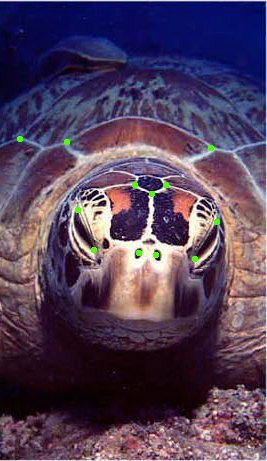
\includegraphics[scale=0.5]{TurtleD1.png}\hspace{0.2cm}
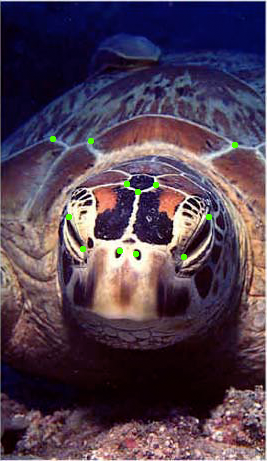
\includegraphics[scale=0.5]{TurtleG1.png}
\end{center}
\vspace{0.5cm}

\subsection{Identification de la matrice fondamentale}

Les points choisis permettent de calculer la matrice fondamentale. Son calcul repose sur l'idée de choisir un point $X_{1}$ sur la première image, puis de déterminer un point objet $X$ se projetant sur ce point image, et finalement de calculer l'image $X_{2}$ de $X$ sur la deuxième image.

Les valeurs de la matrice sont très proches de zéro.



\subsection{Calcul des droites épipolaires}

La matrice fondamentale contient toute les informations nécessaire à la suite des calculs. On peut ainsi calculer pour tout point $X_{1}$ la droite épipolaire correspondante dans la deuxième image, et inversement à un point $X_{2}$ sur la deuxième image, la droite épipolaire sur la première image.

\textbf{Les droites épipolaires s'intersectent en un point : l'épipôle}.

%8 min paires de points de contrôle,  -> calcul matrice fondamentale -> droites épipolaires -> épipole
%plusieurs points qui traquent leur position  à partir de la dérivée de la couleur du pixel ~~
\newpage
\section{Poursuite de cible par flot optique}

\subsection{Introduction}
Le flot optique est le mouvement apparent d'un objet et de ses contours sur une scène, causé par le mouvement entre un observateur et une scène.

\subsection{Mise en place}

Nous avons appliqué un algorithme qui va utiliser plusieurs points de contrôles situés sur les contours de l'objet à suivre. Ces points vont traquer la position des pixels auxquels ils sont rattachés, sur les images suivantes de la séquence, à partir de la dérivé de la couleur des pixels.

\begin{center}
\includegraphics[scale=0.3]{Image000.png}\hspace{0.2cm}
\includegraphics[scale=0.3]{Image034.png}\\
\textit{Les images \texttt{001} et \texttt{034} de la séquence d'images}
\end{center}

L'algorithme doit d'abord être initialisé, puis doit être appelé à chaque nouvelle image de la séquence.

\vspace{2cm}
\section*{Note}
Ces deux travaux pratiques m'ont permis de comprendre le fonctionnement de plusieurs méthodes de traitements d'images qui sont utilisés dans le domaine de la réalité augmentée. Bien que j'ai assimilé le fonctionnement théorique de ces algorithmes, la mise en pratique s'est révélée laborieuse et je n'ai pas obtenu de résultats exploitables à mettre dans un compte-rendu.


\end{document}